%% AMS-LaTeX Created with the Wolfram Language for Students - Personal Use Only : www.wolfram.com

\documentclass{article}
\usepackage{amsmath, amssymb, graphics, setspace}

\newcommand{\mathsym}[1]{{}}
\newcommand{\unicode}[1]{{}}

\newcounter{mathematicapage}
\begin{document}

I.1 \(x-\text{$\pi $y}+\sqrt[3]{5}z=0\) is a linear equation\\
I.2 \(x^2+y^2+z^2=1\) is NOT a linear equation\\
I.3 \(x^{-1}+7y+z=\)\(\left(\text{Sin}\left[\frac{\pi }{9}\right]\right)^2\) is NOT a linear equation\\
I.4 \(x+7y+z=\text{Sin}\left[\frac{\pi }{9}\right]\) is a linear equation\\
I.5 \(3\text{Cos}[x]-4y+z=\sqrt{3}\) is NOT a linear equation\\
I.6 \(\text{Cos}[3]x-4y+z=\sqrt{3}\) is a linear equation

II.7

\begin{doublespace}
\noindent\(\pmb{\text{ContourPlot}[\{x + y \text{==} 0, 2*x + y \text{==} 3\}, \{x, 2, 4\}, \{y, -4, -2\},}\\
\pmb{\text{ContourStyle}\to \{\text{Blue},\text{Orange}\}]}\\
\pmb{\text{(*}}\\
\pmb{
\begin{array}{ll}
 \{ & 
\begin{array}{ll}
 x+y & =0 \\
 2x+y & =3 \\
\end{array}
 \\
\end{array}
\Rightarrow \left(
\begin{array}{ccc}
 1 & 1 & 0 \\
 2 & 1 & 3 \\
\end{array}
\right)\Rightarrow R_2-2R_1\Rightarrow \left(
\begin{array}{ccc}
 1 & 1 & 0 \\
 0 & -1 & 3 \\
\end{array}
\right)\Rightarrow 
\begin{array}{ll}
 \{ & 
\begin{array}{ll}
 x+y & =0 \\
 -y & =3 \\
\end{array}
 \\
\end{array}
}\\
\pmb{y=-3}\\
\pmb{}\\
\pmb{x+y=0}\\
\pmb{x=-(-3)}\\
\pmb{x=3}\\
\pmb{\text{*)}}\\
\pmb{\text{Solve}[\{x + y \text{==} 0,2*x + y \text{==} 3\}, \{x,y\}]}\)
\end{doublespace}

\includegraphics{HWork02_linear_eqs_gr1.eps}

\begin{doublespace}
\noindent\(\{\{x\to 3,y\to -3\}\}\)
\end{doublespace}

II.8

\begin{doublespace}
\noindent\(\pmb{\text{ContourPlot}[\{x - 2*y \text{==} 7, 3*x + y \text{==} 7\}, \{x, 2, 4\}, \{y, -3, -1\},}\\
\pmb{\text{ContourStyle}\to \{\text{Blue},\text{Orange}\}]}\\
\pmb{\text{(*}}\\
\pmb{
\begin{array}{ll}
 \{ & 
\begin{array}{ll}
 x-2y & =7 \\
 3x+y & =7 \\
\end{array}
 \\
\end{array}
\Rightarrow \left(
\begin{array}{ccc}
 1 & -2 & 7 \\
 3 & 1 & 7 \\
\end{array}
\right)\Rightarrow R_2-3R_1\Rightarrow \left(
\begin{array}{ccc}
 1 & -2 & 7 \\
 0 & 7 & -14 \\
\end{array}
\right)\Rightarrow 
\begin{array}{ll}
 \{ & 
\begin{array}{ll}
 x-2y & =7 \\
 7y & =-14 \\
\end{array}
 \\
\end{array}
}\\
\pmb{y=-2}\\
\pmb{}\\
\pmb{x-2y=7}\\
\pmb{x=7+2(-2)}\\
\pmb{x=3}\\
\pmb{\text{*)}}\\
\pmb{\text{Solve}[\{x - 2*y \text{==} 7,3*x + y \text{==} 7\}, \{x,y\}]}\)
\end{doublespace}

\includegraphics{HWork02_linear_eqs_gr2.eps}

\begin{doublespace}
\noindent\(\{\{x\to 3,y\to -2\}\}\)
\end{doublespace}

II.9

\begin{doublespace}
\noindent\(\pmb{\text{ContourPlot}[\{3*x - 6*y \text{==} 3, -x + 2*y \text{==} 1\}, \{x, -3.125, 4.5\}, \{y, -1.75, 1.75\},}\\
\pmb{\text{ContourStyle}\to \{\text{Blue},\text{Orange}\}]}\\
\pmb{\text{(*}}\\
\pmb{
\begin{array}{ll}
 \{ & 
\begin{array}{ll}
 3x-6y & =3 \\
 -x+2y & =1 \\
\end{array}
 \\
\end{array}
\Rightarrow \left(
\begin{array}{ccc}
 3 & -6 & 3 \\
 -1 & 2 & 1 \\
\end{array}
\right)\Rightarrow R_2+\frac{1}{3}R_1\Rightarrow \left(
\begin{array}{ccc}
 3 & -6 & 3 \\
 0 & 0 & 2 \\
\end{array}
\right)\Rightarrow 
\begin{array}{ll}
 \{ & 
\begin{array}{ll}
 3x-6y & =3 \\
 0 & =2 \\
\end{array}
 \\
\end{array}
}\\
\pmb{\text{no} \text{solution}}\\
\pmb{\text{*)}}\\
\pmb{\text{Solve}[\{ 3*x - 6*y \text{==} 3,\text{  }-x + 2*y \text{==} 1\}, \{x,y\}]}\)
\end{doublespace}

\includegraphics{HWork02_linear_eqs_gr3.eps}

\begin{doublespace}
\noindent\(\{\}\)
\end{doublespace}

\end{document}
